\documentclass[tikz]{standalone}
\usepackage{mathtools}
\usepackage{etoolbox}
\usetikzlibrary{intersections}

\newcommand{\drawcsys}[5][0]{
    \def\vstep{#1}
    \def\vxmin{#2}
    \def\vxmax{#3}
    \def\vymin{#4}
    \def\vymax{#5}

	\ifstrequal{#1}{0}{}{%
        \draw[help lines,step=\vstep] (\vxmin,\vymin) grid (\vxmax,\vymax);
    }
    \draw[->,thick] (\vxmin,0) -- (\vxmax,0) node[anchor=north] {$x$};
    \draw[->,thick] (0,\vymin) -- (0,\vymax) node[anchor=east]  {$y$};
}


\begin{document}
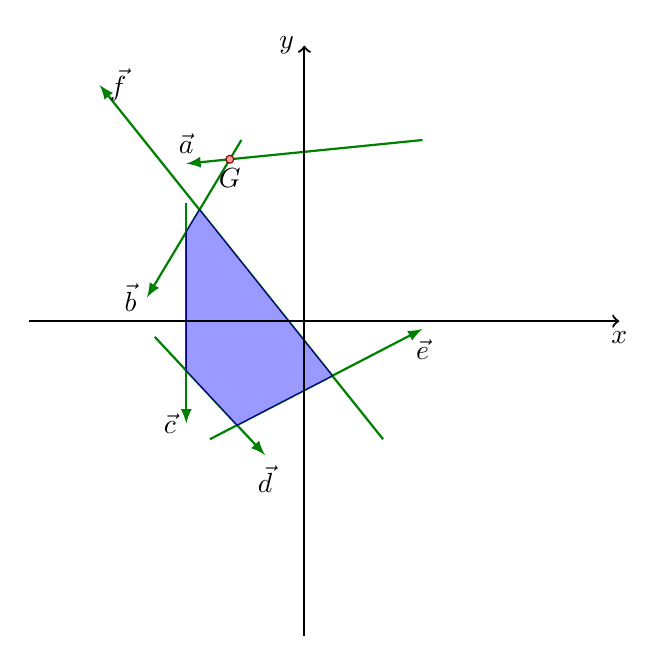
\begin{tikzpicture}[vector/.style={thick,-latex,green!50!black}]
    \draw[name path=veca] [vector] (1.5,2.3) -- (-1.5,2) node [black,above] {$\vec a$};
	\draw[name path=vecb] [vector] (-.8,2.3) -- (-2,.3) node [black,left] {$\vec b$};
	\draw[name path=vecc] [vector] (-1.5,1.5) -- (-1.5,-1.3) node [black,left] {$\vec c$};
	\draw[name path=vecd] [vector] (-1.9,-.2) -- (-.5,-1.7) node [black,below] {$\vec d$};
	\draw[name path=vece] [vector] (-1.2,-1.5) -- (1.5,-.1) node [black,below] {$\vec e$};
	\draw[name path=vecf] [vector] (1,-1.5) -- (-2.6,3) node [black,right] {$\vec f$};

	\path[name intersections={of=veca and vecb}];
	\coordinate [label=270:$G$](G) at (intersection-1);
	\filldraw[draw=red!50!black,fill=red!40!white] (G) circle[radius=.05];

	\path[name intersections={of=vecb and vecc}];
	\coordinate (P0) at (intersection-1);
	\path[name intersections={of=vecc and vecd}];
	\coordinate (P1) at (intersection-1);
	\path[name intersections={of=vecd and vece}];
	\coordinate (P2) at (intersection-1);
	\path[name intersections={of=vece and vecf}];
	\coordinate (P3) at (intersection-1);
	\path[name intersections={of=vecf and vecb}];
	\coordinate (P4) at (intersection-1);

	\filldraw[draw=blue!50!black,fill=blue!40!white] (P0) -- (P1) -- (P2) -- (P3) -- (P4) -- (P0);

	\drawcsys{-3.5}{4}{-4}{3.5}
\end{tikzpicture}
\end{document}
